%!TEX root = ../20XX_Thesis_Example.tex
\section{原稿を書くときに気をつけてほしいこと}\label{sec:points}
Under construction

\subsection{図表}
\textbf{図表は中央揃えで上に配置するようにしてください.}
ネットでは\verb|\includegraphics|コマンドや\verb|tabular|環境の前後を\verb|center|環境で囲むやり方がよく出てきますが,\textbf{現在は推奨されていません.}
\verb|\centering|コマンドを使うようにしましょう.

実験結果のグラフ,イメージ図など挿入するときは基本的に\textbf{pdfを使用してください.}
昔はよくepsを使っていたようですが,pdfの方が図中の文字列を検索できるなどの利点があるようです.
ネット上にはextractbbコマンドでxbbファイルを作れという指示がよく出てきますが,\textbf{古いやり方なので無視してください..}
実験風景や実験器具の写真など,pngやjpgでないといけない場合はそのままで大丈夫です.
pdfの例を\ref{fig:pdf},pngの例を\ref{fig:png},画像を並べた例を\ref{fig:subcaption}に示します.
\begin{figure}[t]
  \centering
  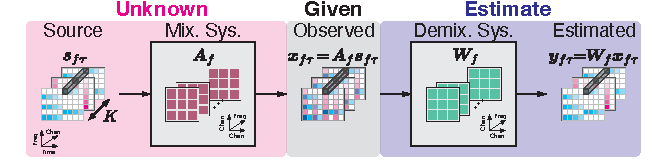
\includegraphics[scale=1.0]{fig/freq-domain-with-notation-en.pdf}
  \caption{pdfの例}\label{fig:pdf}
\end{figure}
\begin{figure}[t]
  \centering
  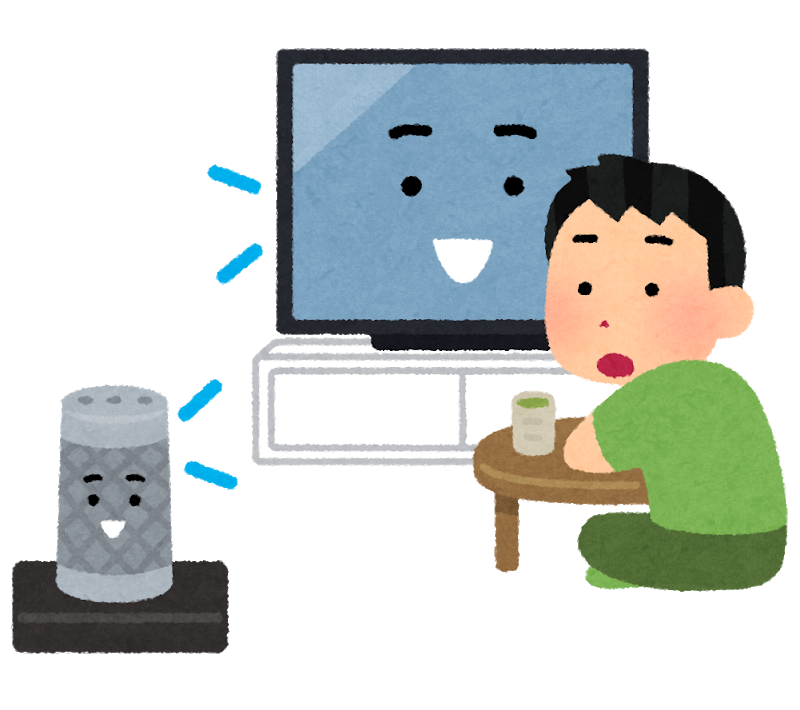
\includegraphics[width=.5\linewidth]{fig/smart_speaker_tv_talk.png}
  \caption{png画像の例}\label{fig:png}
\end{figure}
\begin{figure}[t]
  \centering
  \subcaptionbox{Subfig 1\label{subfig:png}}[.4\linewidth]{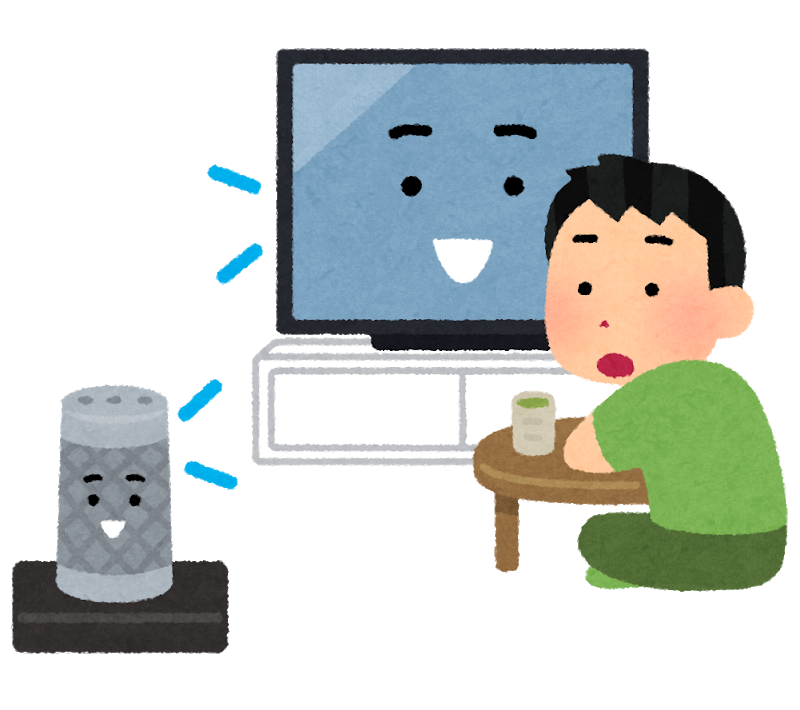
\includegraphics[width=.8\linewidth]{fig/smart_speaker_tv_talk.png}}
  \subcaptionbox{Subfig 2\label{subfig:png}}[.4\linewidth]{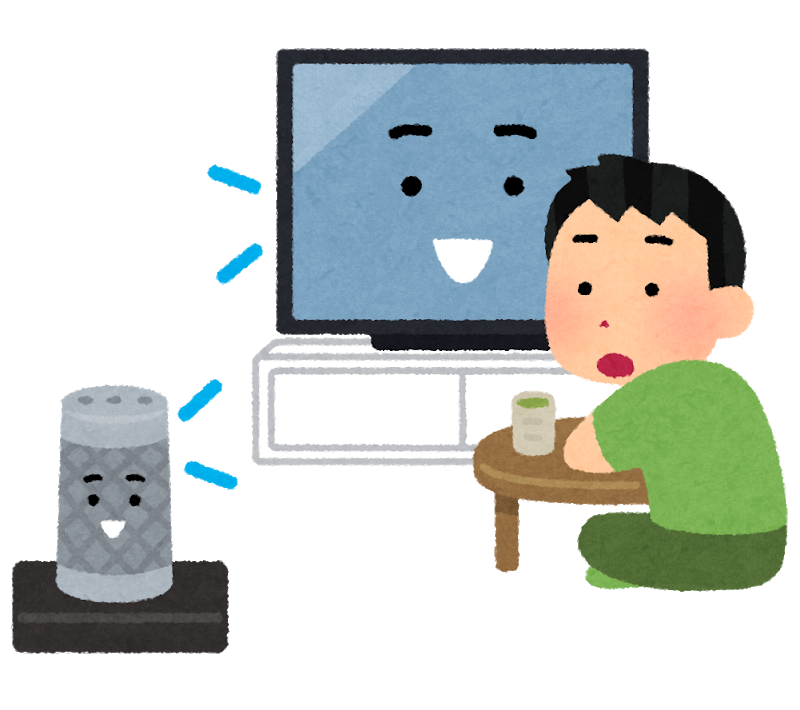
\includegraphics[width=.8\linewidth]{fig/smart_speaker_tv_talk.png}}
  \subcaptionbox{Subfig 3\label{subfig:png}}[.4\linewidth]{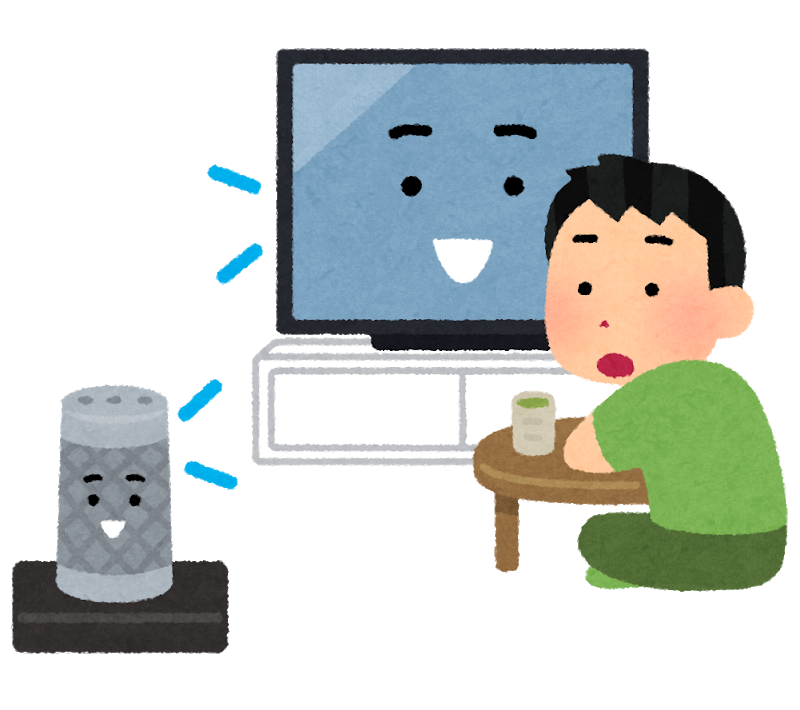
\includegraphics[width=.8\linewidth]{fig/smart_speaker_tv_talk.png}}
  \subcaptionbox{Subfig 4\label{subfig:png}}[.4\linewidth]{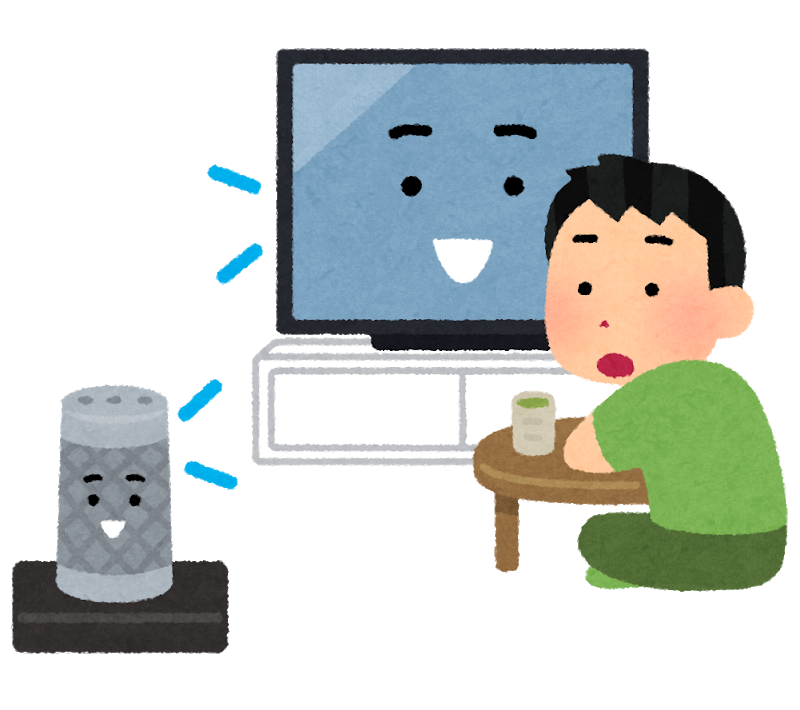
\includegraphics[width=.8\linewidth]{fig/smart_speaker_tv_talk.png}}
  \caption{複数画像の例}\label{fig:subcaption}
\end{figure}

表の例を\ref{tab:table}に示します.
\begin{table}[t]
  \centering
  \caption{表の例}\label{tab:table}
  \begin{tabular}{ll}
    \toprule
    Parameter & Value \\
    \midrule
    STFT frame length & 1024 \\
    STFT frame shift & 512 \\
    STFT window function & Hann \\
    \bottomrule
  \end{tabular}
\end{table}

\subsection{TODO}
その他参考にしてほしいリンク
\begin{itemize}
  \item \url{https://qiita.com/birdwatcher/items/5ec42b35d84d3ee2ffbb}
  \item \url{https://qiita.com/suigin/items/10960e516f2d44f6b6de}
  \item \url{https://qiita.com/Ishotihadus/items/bbbb85f54e6a4e7aaac0}
\end{itemize}

\subsection{TODO}
\begin{itemize}
  \item 数式の細かい書き方
  \item 非推奨のコマンド
  \item 数式環境の使い分け
  \item 独自コマンドの定義
  \item TeX独自の書き方(\verb|`` ''|,en-dash/em-dashなど)についての注意
  \item 擬似コードの書き方
\end{itemize}
